\documentclass[api,pof,pre,12pt,a4paper]{revtex4-1}     
\usepackage{bm}
\usepackage{natbib}
\usepackage{url}
\usepackage[intlimits]{amsmath}
\usepackage{graphicx}
\usepackage{fancyhdr}
\usepackage{amsfonts}
\usepackage{amssymb}
%\usepackage{pstricks}
%\usepackage{pst-coil}
%\usepackage{pst-plot}
\usepackage{hyperref}
\usepackage{float}
\usepackage{subfig}
\usepackage{todonotes}

\newtheorem{theorem}{Theorem}
\newtheorem{prob}{Problem}
\newenvironment{problem}[1]{\begin{prob} {\rm #1} \end{prob}}

%Nadir's Shortcuts
\newcommand{\beqn}{\begin{equation}}
\newcommand{\eeqn}{\end{equation}}
\newcommand{\beqa}{\begin{eqnarray}}
\newcommand{\eeqa}{\end{eqnarray}}
\newcommand{\beqanonum}{\begin{eqnarray*}}
\newcommand{\eeqanonum}{\end{eqnarray*}}
\newcommand{\beqnonum}{\begin{equation*}}
\newcommand{\eeqnonum}{\end{equation*}}
\newcommand{\jump}{\vspace{0.5cm}}
\newcommand{\bbf}{\begin{bf}}
\newcommand{\ebf}{\end{bf}}
%\newcommand{\eqnref}[1]{(\ref{#1})}
\newcommand{\defn}[1]{\begin{bf}\emph{#1}\end{bf}}
\newcommand{\reals}{\ensuremath{\mathbb{R}}}
\newcommand{\complex}{\ensuremath{\mathbb{C}}}
\newcommand{\integers}{\ensuremath{\mathbb{Z}}}
\newcommand{\half}{\ensuremath{\frac{1}{2}}}
\newcommand{\n}{\nonumber}
\renewcommand{\d}{\mathrm{d}}
\newcommand{\del}{\partial}
\newcommand{\dd}{\ensuremath{\, \mathrm{d}}}
\newcommand{\nint}[4]{\int_{#3}^{#4} {#1}\, \mathrm{d}{#2}}
\newcommand{\der}[2]{\frac{\d {#1}}{\d {#2}}}
\newcommand{\parder}[2]{\frac{\del {#1}}{\del {#2}}}
\newcommand{\funder}[2]{\frac{\delta {#1}}{\delta {#2}}}
\newcommand{\Lag}{\mathcal{L}}


% Draft macros
%\newcommand{\TODO}[1]{\marginpar{\raggedright\scriptsize\textbf{TODO:} #1} (\textbf{TODO})}
%\newcommand{\NOTE}[1]{\marginpar{\footnotesize\textbf{NOTE}} (\textbf{#1})}


\oddsidemargin  0.0in
\evensidemargin 0.0in
\textwidth      6.5in
\headheight     15pt
\topmargin      0.0in
\textheight=8.0in
%\setlength{\parindent}{0in}

\lhead{Wavelength competition in modified SH}
\chead{}
\rhead{Gandhi et al.}
%\lfoot{}
%\cfoot{}
%\rfoot{}


%Figures
\newcommand{\FIGmarginalstability}{
\begin{figure}[h]\center
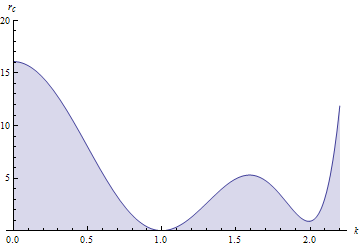
\includegraphics[width=60mm]{MarginalStability.png}
\caption{\label{fig:marginalstability} Linear stability of the modified Swift-Hohenberg equation with $q=2$ and $\delta=.1$.  The shaded region indicates linearly stable parameter regimes of the homogeneous solution with a forcing $r$ for a given wavenumber $k$.}
\end{figure}
}
\newcommand{\FIGbifurcationdiagramA}{
\begin{figure}[h]\center
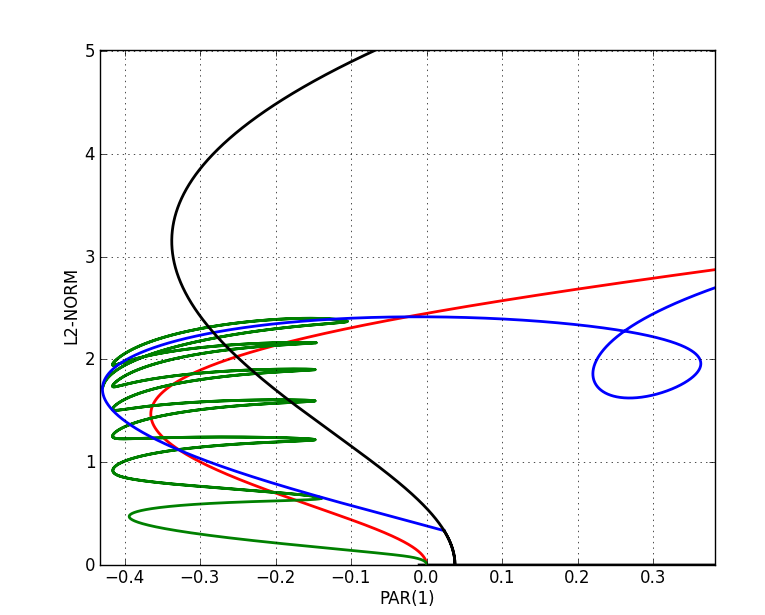
\includegraphics[width=120mm]{BifurcationDiagram1.png}
\caption{\label{fig:bifurcationdiagram1} A Bifurcation diagram for the case that $q=1$ and $\delta=0$, showing a snaking branch that connects two periodic states.}
\end{figure}
}
\newcommand{\FIGbifurcationdiagramB}{
\begin{figure}[h]\center
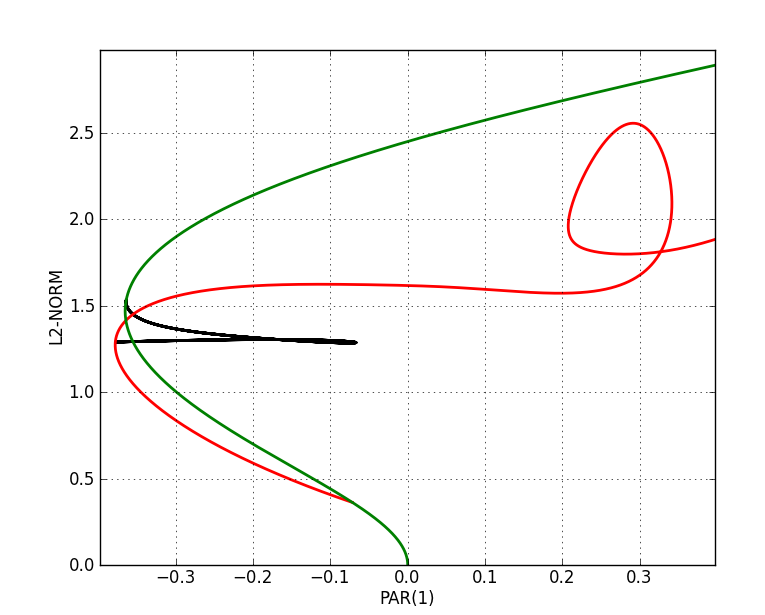
\includegraphics[width=120mm]{BifurcationDiagram2.png}
\caption{\label{fig:bifurcationdiagram2} A Bifurcation diagram for the case that $q=1$ and $\delta=0$, showing the connection of two branches emerging from the $P20$ periodic state.}
\end{figure}
}

\newcommand{\FIGdoubleperiod}{
\begin{figure}[h]
  \begin{center}
    \mbox{
      \subfloat[solution before the loop]{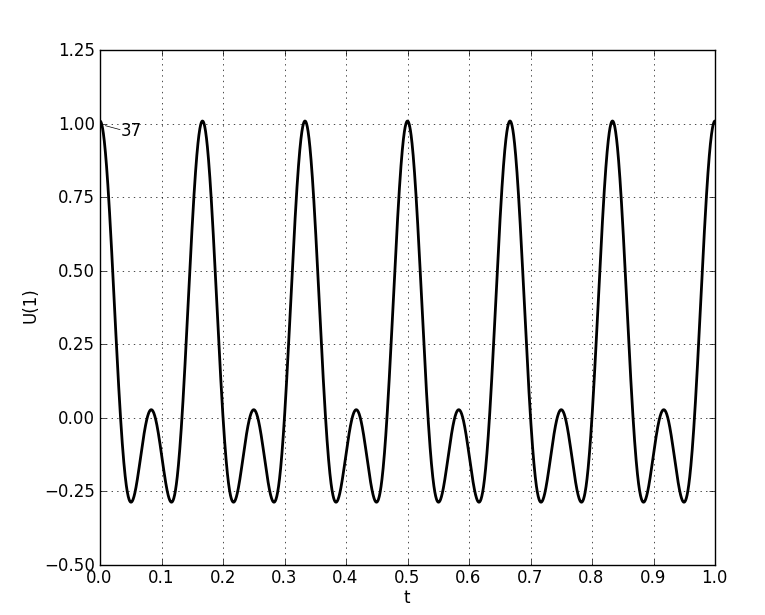
\includegraphics[width=60mm]{dpb24.png}} \quad
      \subfloat[solution after the loop]{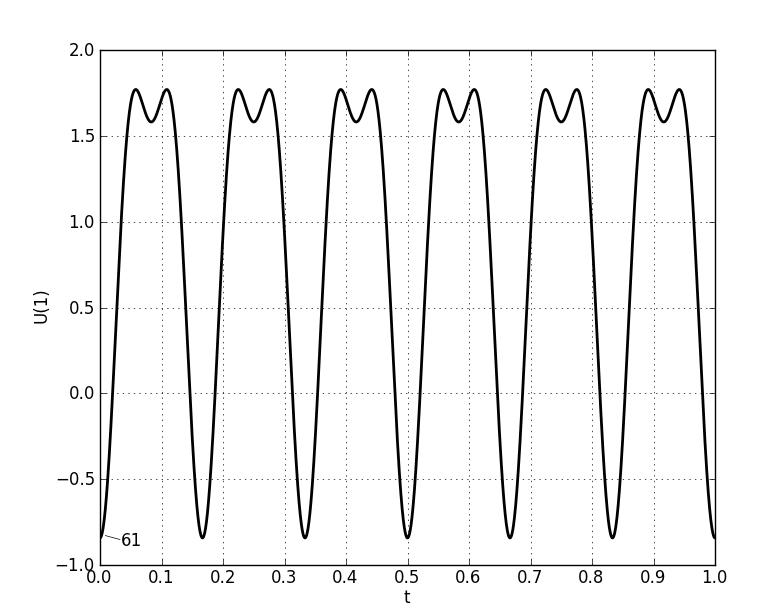
\includegraphics[width=60mm]{dpb24u.png}} 
      }
    \caption{Solutions along periodic branch that bifurcations from $P24$ and connects with the snaking branch from $P20$.}
    \label{fig:doubleperiod1}
  \end{center}
\end{figure}
}

\newcommand{\FIGsnakingA}{
\begin{figure}[h]
  \begin{center}
    
      \subfloat[1]{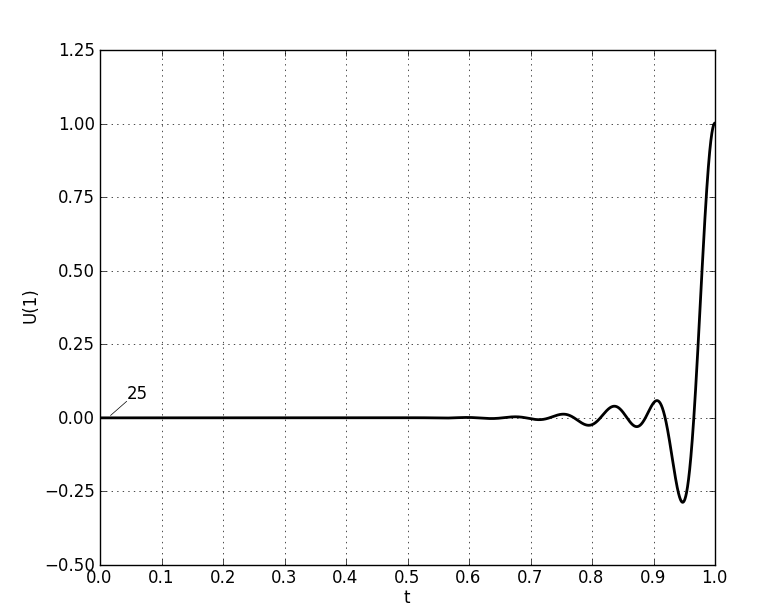
\includegraphics[width=60mm]{sb20a1.png}} \quad
      \subfloat[2]{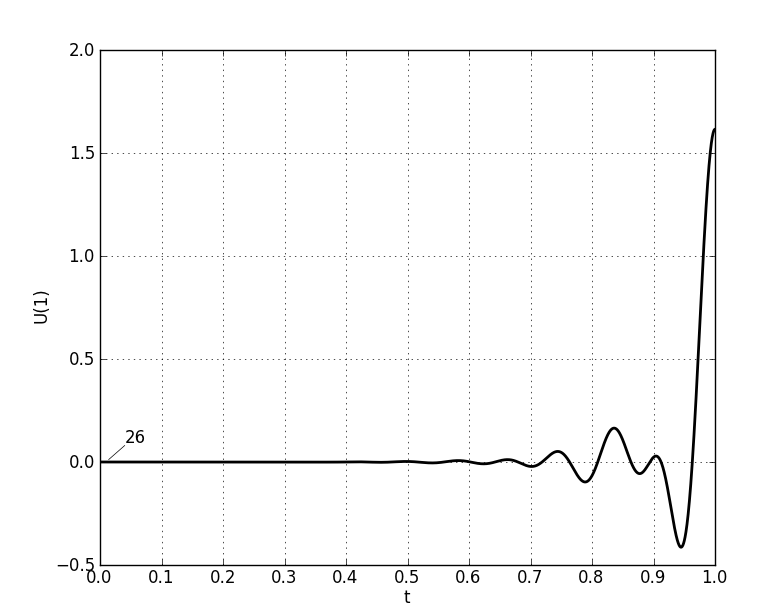
\includegraphics[width=60mm]{sb20a2.png}}\\
      \subfloat[3]{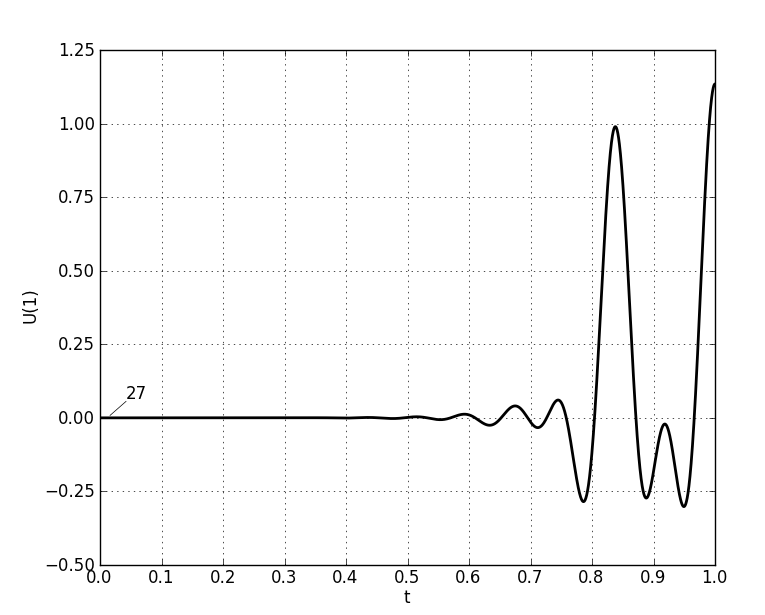
\includegraphics[width=60mm]{sb20a3.png}} \quad
      \subfloat[4]{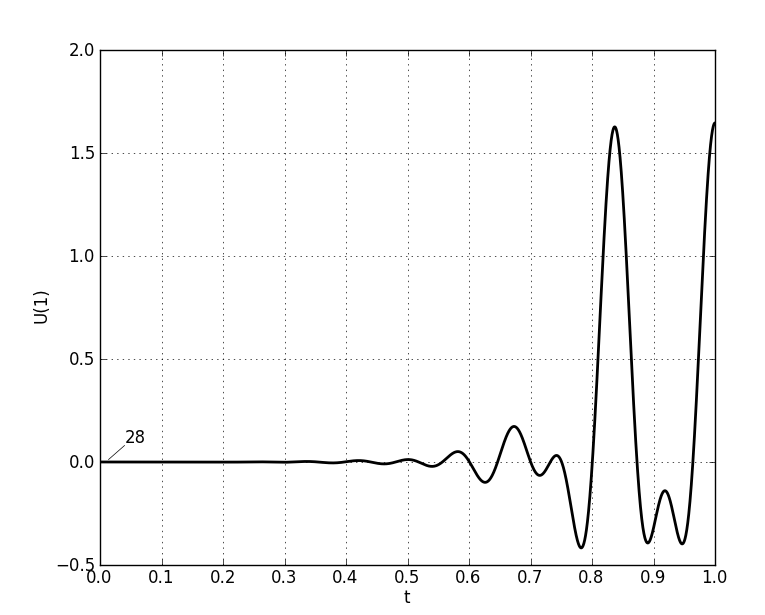
\includegraphics[width=60mm]{sb20a4.png}} 
      
    \caption{Localized solutions along snaking branch that bifurcates from $P20$.}
    \label{fig:snaking1}
  \end{center}
\end{figure}
}


\newcommand{\FIGsnakingmess}{
\begin{figure}[h]
  \begin{center}
    \mbox{
      \subfloat[Example solution from third bifurcation point along $P20$]{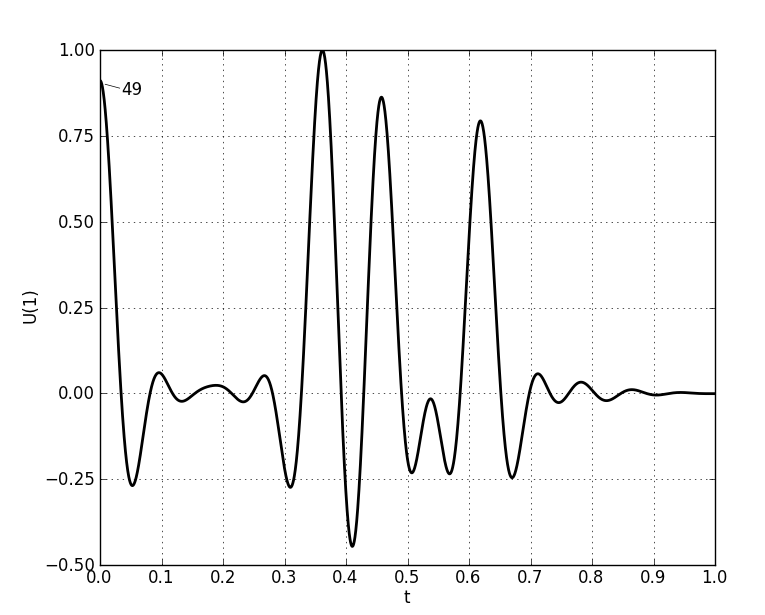
\includegraphics[width=60mm]{sb20cMess.png}} \quad
      \subfloat[Example solution from second bifurcation point along $P24$]{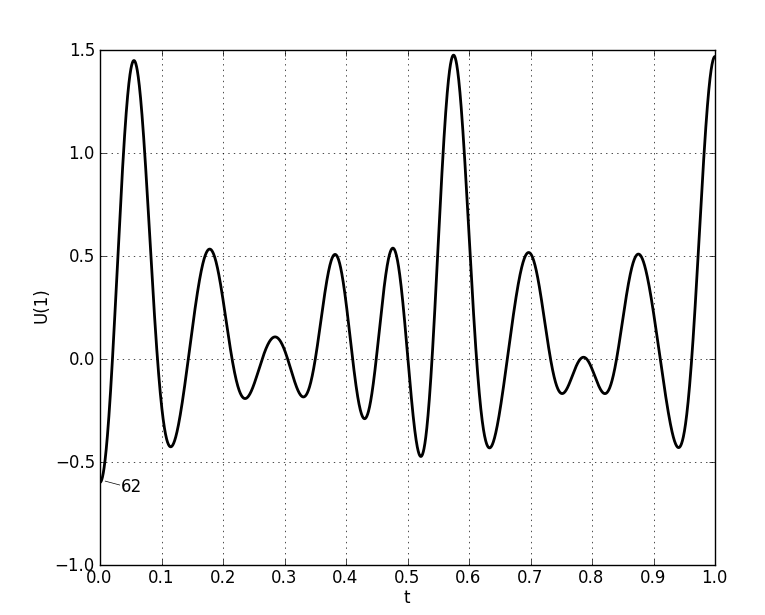
\includegraphics[width=60mm]{sb24bMess.png}} 
      }
    \caption{Examples of solutions with seemingly random pulses. These solutions fall along messy branches that bifurcate from the primary periodic solutions}
    \label{fig:snakingmess1}
  \end{center}
\end{figure}
}

\newcommand{\FIGsnakingB}{
\begin{figure}[h]
  \begin{center}
    
      \subfloat[1]{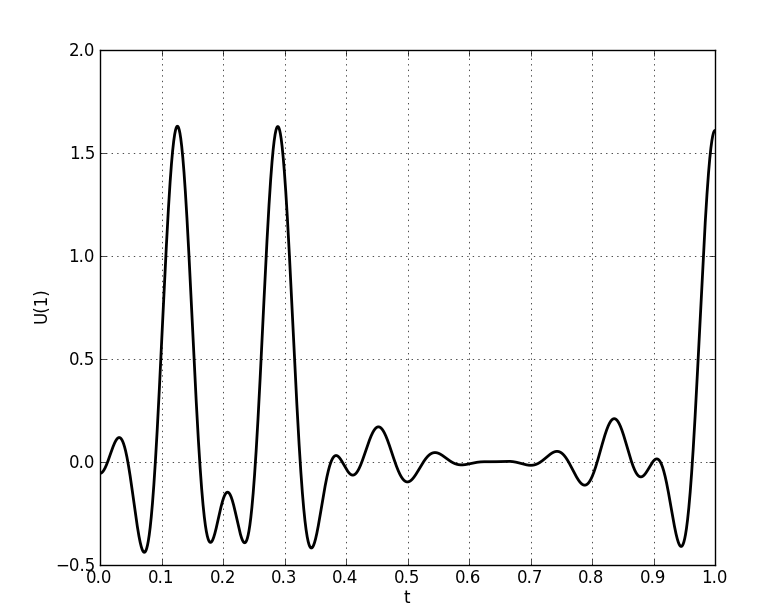
\includegraphics[width=60mm]{sb19a1.png}} \quad
      \subfloat[2]{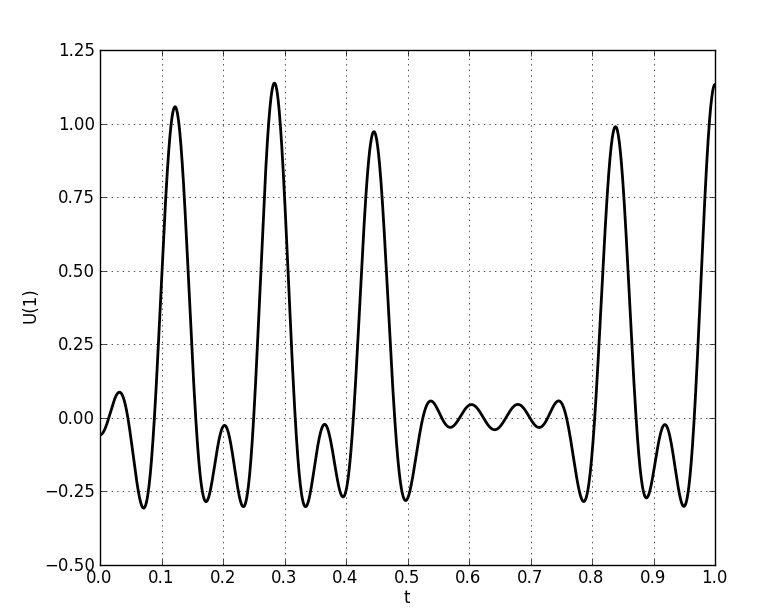
\includegraphics[width=60mm]{sb19a2.png}}\\
      \subfloat[3]{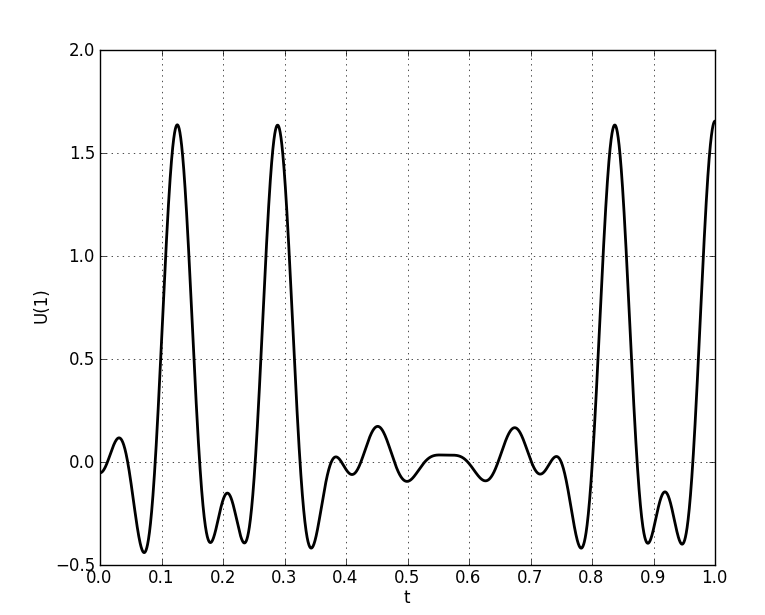
\includegraphics[width=60mm]{sb19a3.png}} \quad
      \subfloat[4]{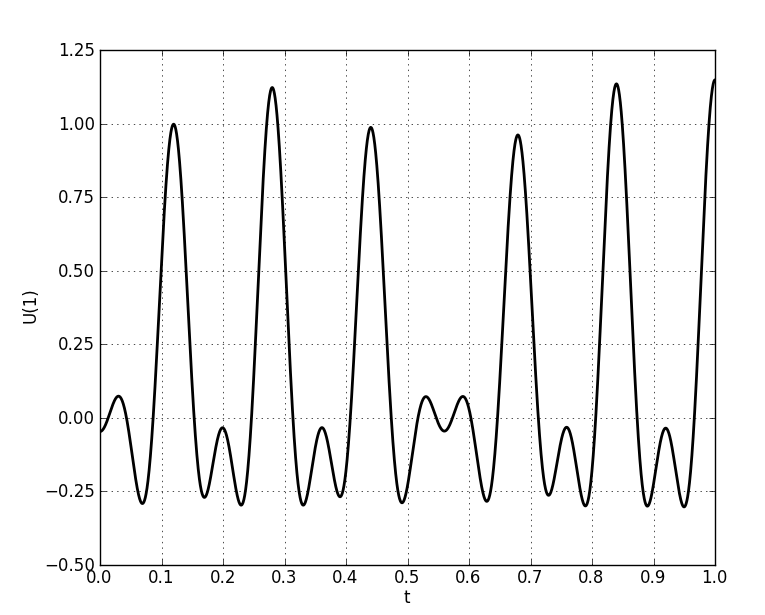
\includegraphics[width=60mm]{sb19a4.png}} 
      
    \caption{Localized solutions along snaking branch that bifurcates from $P19$.}
    \label{fig:snaking19a}
  \end{center}
\end{figure}
}
\newcommand{\FIGbifurcationdiagramC}{
\begin{figure}[h]\center
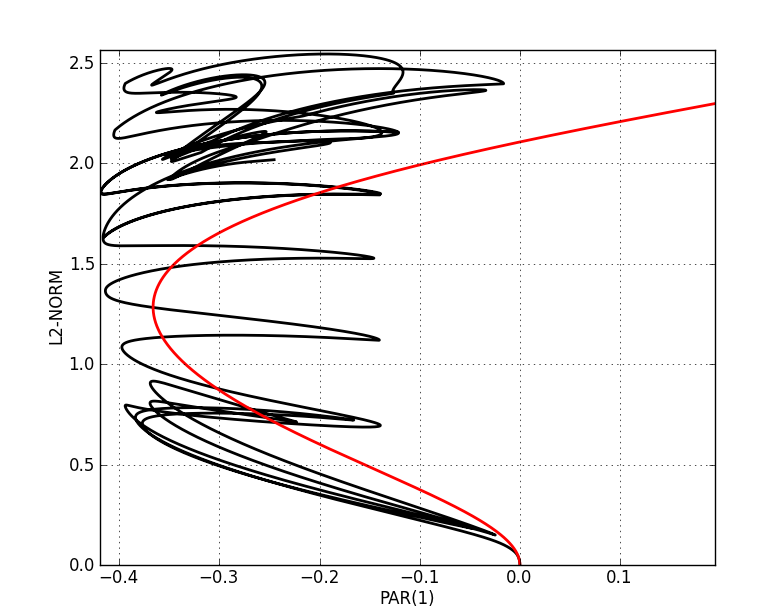
\includegraphics[width=120mm]{sb19a.png}
\caption{\label{fig:bifurcationdiagram19a} A Bifurcation diagram for the case that $q=1$ and $\delta=0$, showing the first snaking branch emerging from the $P19$ periodic state.}
\end{figure}
}


\pagestyle{fancy}
\begin{document}
\preprint{APS/123-QED}

\title{Pattern Formation in a system with competing wavelengths}

\author{Punit Gandhi}
 \email{punit_gandhi@berkeley.edu}
\author{C\'edric Beaume}
\author{Edgar Knobloch}
 \email{knobloch@berkeley.edu}
\affiliation{Department of Physics, University of California, Berkeley CA 94720, USA}

\begin{abstract}
We propose a modified version of the Swift-Hohenberg equation in an attempt to study a situation in which competition between two patterns of different wavelength exist.
\end{abstract}

\maketitle

\section{Introduction}
The Swift-Hohenberg equation serves as a model for pattern formation in a broad range of physical systems.   This equation, which takes the form  
\begin{equation}
u_t= r u-\left(1+\partial_{x}^2\right)^2u+N[u]\label{eq:SH},
\end{equation}
describes the dynamics of a real field $u$ over one spatial dimension in time, where $N$ is some nonlinear function of $u$.  We have rescaled the equation so that the critical wavenumber that defines the natural wavelength of the patterned state is unity.  We will be interested in two possible choices of $N$, namely $N_{23}[u]=bu^2-u^3$ and $N_{35}[u]=b u^3-u^5$.  The strength of the linear forcing term $r$ and the strength of the quadratic nonlinearity $b$ are left as parameters of the system.  

There may be physical systems in which multiple patterned states with different characteristic wavelengths can exist simultaneously.  We would like to develop a model for such a system and study the interaction and competition between these patterned states.  We propose a modification to the Swift-Hohenberg equation in which such competition may be possible:
\begin{equation}
u_t= r u-\left(1+\partial_{x}^2\right)^2 \left[\left(q^2+\partial_{x}^2\right)^2+\delta \right] u+N[u]\label{eq:SHm}.
\end{equation}
Linear stability analysis of this equation results in a marginal stability curve (Fig. \ref{fig:marginalstability}) where two wavelengths can compete with each other.  The first wavelength is  $k=1$, just as in the original SHE (Eq.~\ref{eq:SH}), and the other occurs at 
\beqn
q_*=\frac{1}{2}\sqrt{1+3q^2 \pm\Delta}.
\eeqn
where $\Delta=\sqrt{(q^2-1)^2-8\delta}$ and $+$/ $-$ is used when $q>1$ and $q<1$ respectively.  We note that such solutions exist only when $(q^2-1)^2>8\delta$, which is the condition that there are  local extrema other than $k=1$ in the marginal stability curve.  We must further make the restriction that $\delta>-(q^2-1)^2$ in order that $k=1$ is in fact a local minimum.  If both these conditions are met, there will be a minimum at $q^*$ in addition to 1.  The curve that defines the region of interest to us is also proportional to the marginal stability curve of the original Swift-Hohenberg operator with characteristic wavenumber $q$ and forcing $\delta$.  \todo[inline]{Why is this the case, does it have some physical interpretation?}  This is not a constraining restriction since we will generally be interested in small values of $\delta$.
\FIGmarginalstability
When $\delta=0$, we have that $q_*=q$  and both wavelengths  become unstable at $r=0$. The instability of $q_*$ is shifted for nonzero values of $\delta$ by
\beqn
r_*=\frac{1}{128} \left(3( q^2-1)+\Delta\right)^2 \left( (q^2-1)^2- (q^2-1)\Delta+4 \delta \right).
\eeqn

We will be interested in the case that $\tfrac{8\delta}{(q^2-1)^2}<<1$,  so that the two competing wavelengths will have similar marginal stabilities and can thus compete.  This assumption allows us to approximate $q_*$ and $r_*$ as:
\beqa
q_*&\approx&q\left[1-\frac{\delta}{2q^2(q^2-1)^2}+\frac{\left(9 q^2-1\right) \delta ^2}{8 q^4 \left(q^2-1\right)^3}\right] \\
r_*&\approx& (q^2-1)^2 \delta-\delta^2
\eeqa
We note that the $q=1$ is a degenerate case that may need to be handled separately.  In terms of the our analysis here, $q=1$ requires that $\delta=0$ and in this case, $q_*=q$ and $r_*=0$.  Another interesting regime could be when $q$ is close to one so that we have nearby wavelengths competing. We might also want to consider the case when $q>>1$ (or $q<<1$) so that the wavelengths of the patterns occur on different lengthscales.  This regime is of interest for quasicrystals?

This equation has been studied by Bentley (2012), though with a slightly different parametrization.  The advantage of this parametrization over the one used by Bentley becomes apparent in the small $\delta$ limit.  We see that $q$ is approximately the wavenumber of the second competing pattern, and $\delta$ is proportional to the relative shift between the onsets of the two patterns.   We might also consider a slightly different parametrization in which the $\delta (1-k^2)^2$ is instead $\delta (1-k^2)$, the so-called "Proctor term" (I think).  The advantage of our parametrization is two-fold: (1) the characteristic wavenumber of one of the patterns is exactly one. (2) The relations between $q_*$, $r_*$ and $q$ and $\delta$ are much simpler in our case.    Bentley has looked at this equation as a model for magnetorotational Taylor-Couette flows.  His focus is in the supercritical regime where the patterned states bifurcate from the homogeneous state with a supercritical pitchfork bifurcation.  He is currently working to publish his work.  We don't know what additional work he has done beyond his thesis that his advisor has shared with us.

\section{Variational Structure}
Just as in the case of the original Swift-Hohenberg equation (Eq. \ref{eq:SH}), this modified equation can be expressed in terms of a Lyaponuv functional as 
where
\beqn
F[u]=
\eeqn
This implies that the system will always approach a steady state in time, and we can focus on time-independent solutions to give some insight into the dynamics of the system.

\section{Weakly Nonlinear Analysis}
We would like to look at small amplitude solutions in the neighborhood of the $r=0$ bifurcation where the periodic state branches off of the homogeneous state in the space of steady-state solutions.  We will take a multi-scale approach, defining a slow timescale $T=\epsilon^2t$, and long spatial scale $X=\epsilon x$ so that the derivatives become $\partial_t \rightarrow \partial_t+\epsilon^2\partial_T$ and $\partial_x \rightarrow \partial_x+\epsilon\partial_X$.  We will assume that the system will not change on the fast timescale, so we can neglect the $\partial_t$ term. With some trial and error, it can be seen that the appropriate scaling of forcing strength to probe the dynamics we are interested in will be $r=\epsilon^2 \mu$. In addition, we will choose to scale the shift parameter $\delta\rightarrow\epsilon^2 \delta$ so that the difference in onset of instability for the two wavelengths will be of the same order of the forcing that we consider.  

There are a few issues to consider here, especially after looking at the work of Bentley.  I picked the above scaling to match what is standard in the original Swift-Hohenberg equation.  I had mostly completed this calculation before looking at Bentley's thesis, and noticed that he picked a slightly different scaling.    His large spacial scale goes like  $X=\epsilon^{1/2} x$ instead of  $X=\epsilon x$ .   Considering that we have upped the spatial order of the equation from 4 to 8,  his scaling makes sense because it "keeps the balance between the spatial and time orders the same."   The other thing he does differently that what I have done is to look near the codimension 3 point where $\delta=0$ and $q=1$, whereas I have set up my equations  to be valid for arbitrary (rational) values of q that do not necessarily need to be close together.  I do, however, in this analysis assume that q is of order 1.  Choosing q either very large or small is of interest, and should be done as well.  The cost of my approach is that I require two coupled amplitudes that must be solved whereas Bentley can get a single amplitude equation in one variable.  Since his amplitude varies over length scales of order $\epsilon^{-1/2}$ while mine two amplitudes vary over length scales order $\epsilon^{-1}$, I am guessing the physical explanation is that he is somehow incorporating the beat frequencies from my two amplitudes as a slowly varying modulation?  Since I have gotten so far into my calculation before realizing that I might even consider a different scaling, I decided to go ahead and finish it to see what I get.

One other issue that arises, comes due to my choice of how to write down the equation. As was discussed in the Introduction, $q$ is not actually the wavenumber of the second pattern and yet it is the wavenumber of the leading order problem in this scaling.  The shift in wavenumber happens at a very high order, so maybe it doesn't appear at the order of calculation I'm working at.  I'm guessing that when it does appear, it appears as a correction to the slowly varying amplitude.  The other option is that I should change the form of my solution to include corrections directly to the wavenumber, $u~B e^{i(k_0+\epsilon k_1+...)x}$.  I'm not sure if this is a problem or not yet, but I need to check this a little more carefully.

The linear part of the modified Swift-Hohenberg equation (Eq.~\ref{eq:SHm}), 
\beqn
L= r-\left(1+\partial_{x}^2\right)^2 \left[\left(q^2+\partial_{x}^2\right)^2+\delta \right],
\eeqn
can be expanded as $L=L_0+\epsilon L_1+\epsilon^2 L_2+...$ where:
\begin{subequations}
\begin{align}
L_0 =& -\left(1+\partial_x^2\right)^2 \left(q^2+\partial_x^2\right)^2 \\
L_1 =& -4\left(1+\partial_x^2\right)  \left(q^2+\partial_x^2\right) \left(q^2+1+2 \partial_x^2\right)\partial_x\partial_X \\
L_2 =&- 2 \left[14 \partial_x^6+15  \left(q^2+1\right)\partial_x^4+3 \left(q^4+4 q^2+1\right) \partial_x^2+q^2\left(q^2+1\right)\right] \partial_X^2\nonumber\\  
& \qquad -\delta \left[1+ \left(2+\partial_x^2\right)\partial_x^2\right] +\mu -\partial_T \\
L_3 =& -4   \left[ \left(14 \partial_x^4+10  \left(q^2+1\right)\partial_x^2+q^4+ 4 q^2+1\right)\partial_X^2+\delta\left(1 +\partial_x^2\right)\right]\partial_x \partial_X \\
L_4 =& -\left[\partial_X^2 \left(70 \partial_x^4+30\left(q^2+1\right) \partial_x^2 +q^4 +4 q^2+1\right)+2 \delta\left(1 +3 \partial_x^2 \right) \right] \partial_X^2  \\
L_5=& -4  \left[ \left(3(q^2+1)+14 \partial_x^2\right)\partial_X^2+\delta \right]\partial_x \partial_X^3\\
L_6=& - \left[2 \left(q^2+1+14 \partial_x^2\right)\partial_X^2+\delta \right]\partial_X^4 
\end{align}
\end{subequations}


\subsection{The quadratic-cubic nonlinearity}
We will first consider the case when $N=N_{23}$ so that the modified Swift-Hohenberg equation can be written as $L[u]-N_{23}[u]=0$.  We will assume that the solution can be written as an asymptotic series with the leading term of order $\epsilon$, namely $u=\epsilon u_1 + \epsilon^2 u_2 +\epsilon^2 u_3+...$ 

We can then write out the resulting equation at each order of $\epsilon$ by matching terms at the proper order.
\begin{subequations}
\begin{align}
\mathcal{O}(\epsilon): \:  &-L_0 u_1 =0
\label{eq:msh23o1} \\
\mathcal{O}(\epsilon^2): \: &-L_0 u_2 = L_1 u_1 +b u_1^2
\label{eq:msh23o2} \\
\mathcal{O}(\epsilon^3): \:  &-L_0 u_3 = L_1 u_2 +L_2 u_1 + 2b u_1 u_2-u_1^3
\label{eq:msh23o3}
\end{align}
\end{subequations}
The solution to the $\mathcal{O}(\epsilon)$ equation can be expressed in terms of the yet to be determined complex amplitudes $A_1, B_1$ as:
\beqn
u_1(x,X,T)=A_{11}(X,T)e^{i x} +B_{11}(X,T)e^{i q x} +c.c.
\label{eq:sol23o1}
\eeqn
where $c.c.$ denotes the complex conjugate of the expression written.  The  $\mathcal{O}(\epsilon^2)$ equation has solutions that can be written in the form:
\beqa
u_2(x,X,T)&=&C_{20}(X,T)  \\
&+ &\left[ A_{21}(X,T)e^{i x}+A_{22}(X,T)e^{2 i x} +B_{21}(X,T)e^{i q x} + B_{22}(X,T)e^{2 i q x} +c.c.\right]\nonumber
\label{eq:sol23o2}
\eeqa
Noting that $L_1 u_1=0$, we see that substituting Eqs.~\ref{eq:sol23o1} and ~\ref{eq:sol23o2} into Eq.~\ref{eq:msh23o2} results in the condition
\begin{align}
	0=& \left(2 b (|A_{11}|^2+|B_{11}|^2)-q^4 C_{20} \right) \nonumber \\
 &+\biggl[ \left(b A_{11}^2-9(q^2-4)^2A_{22}\right)e^{2 i x} +\left(b B_{11}^2-9q^4 (1-4q^2)^2 B_{22}\right)e^{2 i q x} \nonumber \\
&+2b B_{11}\left(A_{11}e^{i(q+1)x}+\bar{A}_{11}e^{i(q-1)x} \right)+ c.c.\biggr]
\label{eq:solvability2}
\end{align}
In order to proceed with the analysis, we will eventually need to make some assumptions about the choice of $q$.  We will assume that $q=m/n$ is a rational number where $m$ and $n$ are relatively prime integers. In this case, we want to perform our Fourier analysis on a domain of size $2\pi n$.
We can make use of orthagonality conditions to derive relations between the various amplitudes.  Applying the integral operater $\tfrac{1}{2\pi n}\int_{-n\pi }^{ n\pi} \; \text{d}x$ to Eq.~\ref{eq:solvability2} gives:
\beqn
 \left[2 b (|A_{11}|^2+|B_{11}|^2)-q^4 C_{20} \right] +\delta_{\text{d}}(q-1) \left[2  b B_{11} \bar{A}_{11}+2  b\bar{B}_{11} A_{11} \right]=0
% \left[2 b (|A_{11}|^2+|B_{11}|^2)-q^4 C_{20} \right] +\frac{ \sin(m-n)\pi}{(m-n)\pi} \left[2  b B_{11} \bar{A}_{11}+2  b\bar{B}_{11} A_{11} \right]=0
\eeqn
where $\delta_{\text{d}}$ is the Dirac delta function.
Assuming that $q\neq 1$, this gives a condition that 
\beqn
C_{20}=\frac{2 b}{q^4} (|A_{11}|^2+|B_{11}|^2)
\eeqn
and if $q=1$, we get
\beqn
C_{20}=\frac{2 b}{q^4} (|A_{11}+B_{11}|^2)
\eeqn


Applying $\tfrac{1}{2\pi n }\int_{- n\pi}^{n\pi}  \; \text{d}x\; e^{-ix}$ and $\tfrac{1}{2\pi n }\int_{- n\pi}^{n\pi}  \; \text{d}x\; e^{-i q x}$ give:
\beqn
\delta_{\text{d}}(q-1/2) \left[b B_{11}^2-9q^4 (1-4q^2)^2 B_{22}\right] +\delta_{\text{d}}(q-2) \left[2bB_{11}\bar{A}_{11} \right]=0
%\frac{\sin(2m-n) \pi  }{(2m-n)\pi } \left[b B_{11}^2-9q^4 (1-4q^2)^2 B_{22}\right] +\frac{ \sin (m-2n)\pi }{(m-2n)\pi} \left[2bB_{11}\bar{A}_{11} \right]=0
\eeqn
and
\beqn
\delta_{\text{d}}(q-1/2)\left[2b\bar{B}_{11} A_{11} \right]  +\delta_{\text{d}}(q-2) \left[b A_{11}^2-9 (q^2-4)^2 A_{22}\right]=0
%\frac{\sin(2m-n) \pi  }{(2m-n)\pi }\left[2b\bar{B}_{11} A_{11} \right]  +\frac{ \sin (m-2n)\pi }{(m-2n)\pi} \left[b A_{11}^2-9 (q^2-4)^2 A_{22}\right]=0
\eeqn
respectively.  These equations are trivially solved, unless $q=2$ or $q=1/2$.  

Applying $\tfrac{1}{2\pi n}\int_{-n \pi}^{ n\pi}  \; \text{d}x\; e^{2i x}$  and $\tfrac{q}{2\pi n}\int_{-n\pi}^{n\pi}  \; \text{d}x\; e^{2iqx}$ give:
\begin{align}
0=&\left[b A_{11}^2-9 (q^2-4)^2 A_{22}\right]\nonumber \\
&+\delta_{\text{d}}(q-1) \left[2bB_{11}A_{11}+b B_{11}^2-9q^4 (1-4q^2)^2 B_{22}\right]+\delta_{\text{d}}(q-3) \left[2bB_{11}\bar{A}_{11}\right]
%\left[b A_{11}^2-9 (q^2-4)^2 A_{22}\right]+\frac{ \sin(m-n)\pi }{(m-n)\pi} \left[2bB_{11}A_{11}\right]
%+\frac{\sin2(m-n) \pi  }{2(m-n)\pi} \left[b B_{11}^2-9q^4 (1-4q^2)^2 B_{22}\right]\nonumber \\
%+\frac{ \sin(m-3n)\pi }{(m-3n)\pi} \left[2bB_{11}\bar{A}_{11}\right]=0
\end{align}
and
\begin{align}
0=&\left[b B_{11}^2-9q^4 (1-4q^2)^2 B_{22}\right]\nonumber \\
&+\delta_{\text{d}}(q-1) \left[2bB_{11}A_{11}+b A_{11}^2-9 (q^2-4)^2 A_{22}\right]+\delta_{\text{d}}(q-1/3) \left[2b\bar{B}_{11}A_{11}\right]
%\left[b B_{11}^2-9q^4 (1-4q^2)^2 B_{22}\right]+\frac{ \sin(m-n)\pi }{(m-n)\pi} \left[2bB_{11}A_{11}\right]
%+\frac{\sin2(m-n) \pi  }{2(m-n)\pi q} \left[b A_{11}^2-9 (q^2-4)^2 A_{22}\right]\nonumber \\
%+\frac{ \sin(3m-n)\pi }{(3m-n)\pi} \left[2b\bar{B}_{11}A_{11}\right]=0
\end{align}
respectively.  In the case that $q=1$, we again get the solution consistent with combining the two amplitudes into a single variable.  The $q=3,1/3$ cases give a coupling between the two amplitudes in this equation, and all other cases give:
\beqn
A_{22}=\frac{bA_{11}^2}{9 (q^2-4)^2} \qquad B_{22}=\frac{bB_{11}^2}{9q^4 (1-4q^2)^2}
\eeqn

Now, going on to the $\mathcal{O}(\epsilon^3)$, we can write down the solution in the form:
\beqa
u_3(x,X,T)=C_{30}(X,T)  + \biggl[ &A&_{31}(X,T)e^{i x}+A_{32}(X,T)e^{2 i x}+A_{33}(X,T)e^{3 i x}\\ 
+&B&_{31}(X,T)e^{i q x} + B_{32}(X,T)e^{2 i q x}+B_{33}(X,T)e^{3 i q x} +c.c.\biggr]\nonumber
\label{eq:sol23o3}
\eeqa

In order to get the solvability conditions that determine the leading order amplitudes, we need only look at the following two  projections of this equation:   $\tfrac{1}{2\pi n}\int_{-n\pi}^{n\pi}  \; \text{d}x\; e^{-ix}$ and $\tfrac{q}{2\pi n}\int_{- n\pi}^{n \pi}  \; \text{d}x\; e^{-iqx}$.  The conditions will come from forcing these projections that result in resonance terms to vanish.  Leaving $q$ as an arbitrary rational number makes the calculation more difficult because we must now calculate more terms of the equation as they may have a component along these directions.  We will calculate each term in the equation, and then look at the final equations resulting from the projections.  An alternative way to look at this problem is to make use of the Fredhom alternative theorem, which will result in basically the same calculation.

We first not that $L_0 u_3$ and $L_1 u_2$ cannot have a component along the directions we are looking for as both directions lie completely in the kernels of these operators.  We must therefore compute $L_2 u_1$ and the two nonlinear terms in order to find the solvability condition.
\begin{align}
L_2 u_1=&\left[4\left(q^2-1\right)^2 \partial_X^2 A_{11}+\mu A_{11}-\partial_T A_{11}\right]e^{i x}\nonumber \\
+&\left[4q^2\left(q^2-1\right)^2 \partial_X^2 B_{11}+\left(\mu-\delta (q^2-1)^2\right) B_{11}-\partial_T B_{11}\right]e^{i q x} \nonumber\\
+&c.c
\end{align}
\begin{align}
2 b u_1 u_2=2b\biggr[&A_{11}A_{22} e^{3ix}+A_{11}A_{21} e^{2ix}+\left(A_{11}C_{20}+A_{22}\bar{A}_{11}\right) e^{ix}+A_{11}\bar{A}_{21}\nonumber \\+&B_{11}B_{22} e^{3iqx}+B_{11}B_{21} e^{2iqx}+\left(B_{11}C_{20}+B_{22}\bar{B}_{11}\right) e^{iqx}+B_{11}\bar{B}_{21}\nonumber \\
+&\left(A_{11}B_{21}+B_{11}A_{21}\right) e^{i(q+1)x}+\left(\bar{A}_{11}B_{21}+B_{11}\bar{A}_{21}\right) e^{i(q-1)x}\nonumber \\
+&A_{22}B_{11} e^{i(q+2)x}+\bar{A}_{22}B_{11} e^{i(q-2)x}+A_{11}B_{22} e^{i(2q+1)x}+\bar{A}_{11}B_{22} e^{i(2q-1)x}\nonumber \\
+&c.c.\biggr]
\end{align}
\begin{align}
-u_1^3=-\biggl[&A_{11}^3 e^{3ix}+\left(3|A_{11}|^2A_{11}+6|B_{11}|^2A_{11}\right) e^{ix}\nonumber\\
+&B_{11}^3 e^{3iqx}+\left(3|B_{11}|^2B_{11}+6|A_{11}|^2B_{11}\right) e^{iqx}\nonumber\\
+&3A_{11}^2 B_{11} e^{i(q+2)x}+3\bar{A}_{11}^2 B_{11} e^{i(q-2)x}+3A_{11}B_{11}^2  e^{i(2q+1)x}+3\bar{A}_{11}B_{11}^2  e^{i(2q-1)x}\nonumber\\
+&c.c.\biggr]
\end{align}
The final solvability conditions become:
\begin{align}
\left[\left(4\left(q^2-1\right)^2 \partial_X^2 A_{11}+\mu A_{11}-\partial_T A_{11}\right)+2b\left(A_{11}C_{20}+A_{22}\bar{A}_{11}\right)-\left(3|A_{11}|^2A_{11}+6|B_{11}|^2A_{11}\right)\right]\nonumber\\
+\delta_{\text{d}}(q-1)\left[\left(4q^2\left(q^2-1\right)^2 \partial_X^2 B_{11}+\left(\mu-\delta (q^2-1)^2\right) B_{11}-\partial_T B_{11}\right)+2b\left(B_{11}C_{20}+B_{22}\bar{B}_{11}\right) -\left(3|B_{11}|^2B_{11}+6|A_{11}|^2B_{11}\right)\right]
\end{align}

If $q\neq 1,2,1/2,3, 1/3$, then the equations become
\begin{align}
\dot{A}&=\mu A+a  A''-\alpha|A|^2A-\gamma|B|^2 A\\
\dot{B}&=\left(\mu-\frac{\delta a}{4}\right) B+q^2 a  B''-\beta|B|^2B-\gamma|A|^2 B
\end{align}
where $a=4(q^2-1)^2$, $\alpha=3-\tfrac{4 b^2}{q^4}-\tfrac{2 b^2}{9(q^2-4)^2}$, $\beta=3-\tfrac{4 b^2}{q^4}-\tfrac{2 b^2}{9q^2(1-4q^2)^2}$, and $\gamma=6-\frac{4 b^2}{q^4}$. We see from this equation that in the $q=1$ case the spatial derivative term vanishes, and this would have been prevented if we used the spatial scaling of Bentley.

We can gain some insight into these coupled equations by rewriting the amplitudes in terms of polar coordinates as $A=r e^{i\theta}$ and $b= s e^{i\phi}$.  Using these variables, the two complex equations can be written as the following 4 real equations:
\begin{subequations}
\begin{align}
\dot{r}=&\mu r + a(r'' - r\theta'^2) -\alpha r^3-\gamma s^2 r
\label{eq:rpolar} \\
r^2\dot{\theta}=&a(r^2\theta')'
\label{eq:thpolar}\\
\dot{s}=&(\mu-\delta a/4) s + q^2 a(s'' - s\phi'^2) -\beta s^3-\gamma r^2 s
\label{eq:spolar}\\
s^2\dot{\phi}=&q^2 a (s^2\phi')'
\label{eq:phpolar}
\end{align}
\end{subequations}
If we focus on time-independent solutions, we can now use the standard trick of mapping the above equations onto a problem of particles in a central potential.  In this case there are two particles in the potential that are coupled together.  The angular momentum of each particle $l_A=r^2\theta'$ and $l_B=s^2\phi'$ are constants of the motion along with the total energy of the system $h=h_A+h_B - h_c$.  Here the energy of the two particles are 
\begin{subequations}
\begin{align}
h_A=&\frac{1}{2} a r'^2 +\frac{1}{2}\mu r^2 + \frac{al_A^2}{2r^2}-\frac{\alpha}{4}r^4
\label{eq:hA} \\
h_B=&\frac{1}{2}q^2 a s'^2 +\frac{1}{2}(\mu-\delta a/4) s^2 + \frac{q^2al_B^2}{2s^2}-\frac{\beta}{4}s^4
\label{eq:hBr}
\end{align}
\end{subequations}
and the coupling term is $h_c=\frac{1}{2}\gamma r^2 s^2$.  In these new variables, the equations of motion become
\begin{subequations}
\begin{align}
h_A'=&\gamma s^2r r'\\
h_B'=&\gamma r^2 s s'\\
l_A'=&0\\
l_B'=&0
%\label{eq:msh23o3}
\end{align}
\end{subequations}


\subsection{The cubic-quintic nonlinearity}


\section{Weakly Nonlinear Analysis REDO}
In this section, we consider the scaling analogous to what Bentley did in which the long spatial scale is defined by $x=\epsilon^{1/2}X$ instead of $x=\epsilon X$ as in the previous section.  All other scalings are identical to the previous section.
The linear part of the modified Swift-Hohenberg equation (Eq.~\ref{eq:SHm}), 
\beqn
L= r-\left(1+\partial_{x}^2\right)^2 \left[\left(q^2+\partial_{x}^2\right)^2+\delta \right],
\eeqn
can be expanded as $L=L_0+\epsilon^{1/2} L_{1/2}+\epsilon L_1+\epsilon^{3/2} L_{3/2}+\epsilon^2 L_2+...$ where:
\begin{subequations}
\begin{align}
L_0 =& -\left(1+\partial_x^2\right)^2 \left(q^2+\partial_x^2\right)^2 \\
L_{1/2} =& -4\left(1+\partial_x^2\right)  \left(q^2+\partial_x^2\right) \left(q^2+1+2 \partial_x^2\right)\partial_x\partial_X \\
L_1 =&- 2 \left[14 \partial_x^6+15  \left(q^2+1\right)\partial_x^4+3 \left(q^4+4 q^2+1\right) \partial_x^2+q^2\left(q^2+1\right)\right] \partial_X^2\\  
L_{3/2} =& -4   \left[ 14 \partial_x^4+10  \left(q^2+1\right)\partial_x^2+q^4+ 4 q^2+1\right]\partial_x \partial_X^3 \\
L_2 =& -\left[ 70 \partial_x^4+30\left(q^2+1\right) \partial_x^2 +q^4 +4 q^2+1\right]\partial_X^4-\delta\left(1 +\partial_x^2\right)+\mu-\partial_T  \\
L_{5/2} =& -4 \left[ \left(3(q^2+1)+14 \partial_x^2\right)\partial_X^4+\delta(1 +\partial_x^2) \right] \partial_x \partial_X  \\
L_{3} =& -2 \left[ \left(q^2+1+14 \partial_x^2\right)\partial_X^4 +\delta(1 +3 \partial_x^2) \right] \partial_X^2 
\end{align}
\end{subequations}

\subsection{The quadratic-cubic nonlinearity}
We will first consider the case when $N=N_{23}$ so that the modified Swift-Hohenberg equation can be written as $L[u]+N_{23}[u]=0$.  We will assume that the solution can be written as an asymptotic series with the leading term of order $\epsilon$, namely $u=\epsilon u_1 + \epsilon^{3/2} u_{3/2} +\epsilon^2 u_2+...$ 

We can then write out the resulting equation at each order of $\epsilon$ by matching terms at the proper order.
\begin{subequations}
\begin{align}
\mathcal{O}(\epsilon): \:  &-L_0 u_1 =0
\label{eq:msh23o1b} \\
\mathcal{O}(\epsilon^{3/2}): \: &-L_0 u_{3/2} = L_{1/2} u_1 
\label{eq:msh23o15b} \\
\mathcal{O}(\epsilon^2): \:  &-L_0 u_2 = L_{1/2} u_{3/2} +L_1 u_1 +b u_1^2
\label{eq:msh23o2b}\\
\mathcal{O}(\epsilon^{5/2}): \:  &-L_0 u_{5/2} = L_{1/2} u_{2} +L_1 u_{3/2}+ L_{3/2} u_1 +2b u_1 u_{3/2}
\label{eq:msh23o25b}\\
\mathcal{O}(\epsilon^{3}): \:  &-L_0 u_{3} = L_{1/2} u_{5/2} +L_1 u_{2}+ L_{3/2} u_{3/2}+L_2 u_1   +b u_{3/2}^2+2b u_1 u_2 -u_1^3
\label{eq:msh23o25b}
\end{align}
\end{subequations}

The solution to the $\mathcal{O}(\epsilon)$ equation can be expressed in terms of the yet to be determined complex amplitudes $A_{11}, B_{11}$ as:
\beqn
u_1(x,X,T)=A_{11}(X,T)e^{i x} +B_{11}(X,T)e^{i q x} +c.c.
\label{eq:sol23o1}
\eeqn
Furthermore, since $L_{1/2} u_1=0$, we can absorb $u_{3/2}$ into $u_1$ as a correction. 

For the next order in $\epsilon$,$\mathcal(\epsilon^2)$ , we see that $L_{1/2} u_{3/2}$ vanishes, and will assume the following form for $u_2$:
\beqa
u_2(x,X,T)&=&C_{20}(X,T)  \\
&+ &\left[ A_{21}(X,T)e^{i x}+A_{22}(X,T)e^{2 i x} +B_{21}(X,T)e^{i q x} + B_{22}(X,T)e^{2 i q x} +c.c.\right]\nonumber
\label{eq:sol23o2}
\eeqa

The resulting condition becomes:
\begin{align}
	0=& \left(2 b (|A_{11}|^2+|B_{11}|^2)-q^4 C_{20} \right) \nonumber \\
&+\biggl[ 4(q^2-1)^2\left( A_{11}''e^{ix}+q^2 B_{11}''e^{iqx} \right)\nonumber \\
 &+\left(b A_{11}^2-9(q^2-4)^2A_{22}\right)e^{2 i x} +\left(b B_{11}^2-9q^4 (1-4q^2)^2 B_{22}\right)e^{2 i q x} \nonumber \\
&+2b B_{11}\left(A_{11}e^{i(q+1)x}+\bar{A}_{11}e^{i(q-1)x} \right)+ c.c.\biggr]
\label{eq:solvability2}
\end{align}
In the case that $q\neq 1$, we see that this requires the leading order amplitudes to satisfy $A_{11}''=B_{11}''=0$, which implies that they must be constants if we assume a finite value at $\pm \infty$ for the boundary conditions.  This choice of scaling works well when $q=1$ as is demonstrated in Bentley's thesis, but does not seem to produce useful results in the more general case. \todo[inline]{Can I modify this scaling slightly or add an additional parameter that appears at this order to cancel out the problematic terms here?  Would an additional time or length scale help, and if so, what would it represent physically?  }





\section{Numerical Results}
The steady state solutions of this system as a function of the forcing strength $r$ can be found by numerical continuation.  Auto was used to compute the below bifurcation diagram and solutions.  We have used a domain size of 20 wavelengths for these simulations, but made use of the reflection symmetry to only simulate half (i.e. our simulation had a spatial size of 20$\pi$).  

\subsection{The one-wavelength case}
The case that $q=1$ and $\delta=0$ is the simplest case to consider since there is only one characteristic wavelength to the problem, namely 1.  We set the nonlinearity parameter to $b=1.8$ as was done by Burke et. al for the original SHE.    We already see a very interesting bifurcation diagram here (Fig.~\ref{fig:bifurcationdiagram1}).
\FIGbifurcationdiagramA
The periodic branch bifurcating from the homogeneous solution at $r=0$ has 20 periods and will be called $P20$.  The first secondary bifurcation from $P20$, forms a snaking branch of one-pulse localized states like the ones shown in Fig.~\ref{fig:snaking1}.
\FIGsnakingA
This branch eventually reconnects to another periodic branch that does not have a constant amplitude and has 12 periods in the domain (See Fig.~\ref{fig:doubleperiod1}).
\FIGdoubleperiod
This periodic solution does not bifurcate from the homogeneous solution, but from the $P24$ periodic branch.  It also has a loop in it, where the solution structure inverts so that the small oscillation are on the top instead of the bottom. The bifurcation is  actually the third branch point along the $P24$ branch if followed starting from the homogeneous solution.  The previous two branches along $P24$ are quite messy with seemingly randomly positioned pulses (See Fig.~\ref{fig:snakingmess1} for an example).
\FIGsnakingmess  
Additionally, we have looked at the solutions formed at the next two bifurcation points along the $P20$ periodic branch.  The second branch snakes with two-pulse localized states while the third branch is messy with seemingly randomly distributed pulses.

Another example of where a  multipulse state branch connects to a secondary periodic state branch is shown in Fig.~\ref{fig:bifurcationdiagram2}.  In this case, a five pulse state grows into the secondary periodic state upon each pulse doubling in size.  Note that this situation is slightly different in that both branches come from the same primary periodic branch.  It is also interesting to note that another five pulse branch appears below the periodic ( or ten pulse) branch, but does not connect as far as I've followed it. The secondary periodic branch with 10 periods shown in this figure contains a loop near $r=0.3$ just as the secondary periodic branch with 12 periods did in Fig.~\ref{fig:bifurcationdiagram1}.  
\FIGbifurcationdiagramB

There are several periodic solutions branching from the homogenous state between $P20$ and $P24$.  By looking at the secondary branches from these periodic states, we hope to see a pattern start to emerge with the location of multipulse states.  Note that we only track multipulse states in which all pulses are identical.  The table below lists in order, the periodic solutions along the diagram from in order of increasing forcing.  We would like to note that we can also interpret the periodic solution shown in Fig.~\ref{fig:doubleperiod1} as a twelve pulse state that just happens to exactly fill the simulation domain.  There are several solutions of this type that can be seen as a multipulse state with half the number of pulses as the periodic branch from which it emerges, or as a periodic solution with twice the wavelength of the branch from which it emerges.  



\begin{table}[ht]
\caption{Cascade of secondary multipulse branches that bifurcate from periodic states.} % title of Table
\centering % used for centering table
\begin{tabular}{c | c c c c c c c c c c} % centered columns (4 columns)
\hline\hline %inserts double horizontal lines
 Branch \# &\multicolumn{10}{c}{ Primary branch}\\
\hline  %\\  %[0.5ex] % inserts table 
%heading
10 	&\textbf{10p} &??		&??		&??		&??		&??		&??		&??		&??		&??	\\
9	&      		&??		&??		&??	 	&??		&??		&??		&??		&??		&??	\\
8	&4p  		&		&		&??	 	&??		&??		&??		&??		&??		&??	\\
7	&      		&		&3p		&??	 	&\textbf{11p}	&??		&??		&??		&??		&??	\\
6	& 2p    		&		&		&\textbf{9p} 	&2p		&??		&??		&		&		&??	\\
5	&\textbf{5p}  	&		&\textbf{7p}	&2p	 	&		&		&		&4p		&		&??	\\
4	&\textbf{4p} 	&		&3p		&	 	&2p		&		&		&		&3p		&??	\\
3	&      		&		&		&\textbf{6p} 	&		&		&		&2p		&		&\textbf{12p}	\\
2	&\textbf{2p} 	&		&		&	 	&2p		&		&		&		&5p		&	\\
1	&\textbf{1p}  	&		&\textbf{3p}	&2p	 	&		&		&		&\textbf{8p}	&3p		&2p	\\
\hline % inserts single horizontal line
 	&$P20$	&$P19$	&$P21$	&$P18$	&$P22$	&$P17$	&$P23$	&$P16$	&$P15$	&$P24$ \\ [1ex] % [1ex] adds vertical spac
\hline %inserts single line
\end{tabular}
\label{table:multipulse} % is used to refer this table in the text
\end{table} 

Following the homogeneous solution branch, we see a series of periodic states bifurcate as the forcing increases.  Each of these branches is labeled by the number of wavelengths that fit into the domain, and the sequence is shown in Table \ref{table:multipulse}.  Secondary bifurcations occur along each of these periodic branches as they are followed away from the homogeneous solution.  Studying the solutions along these secondary branches shows a cascade of multipulse solutions that have a very regular pattern.  The first periodic branch, $P20$ has  one-pulse solution branching off of the first bifurcation point, and then a two pulse solution off of the second one.  The pattern continues as you continue up the branch, except that the nth bifurcation produces an n-pulse state only if n is a factor of the number of periods of  on the branch (namely 20).  The next periodic branch begins with a two-pulse state at the first bifurcation point and increases as one follows the periodic branch up.  The pattern continues so that the next branch starts with a three-pulse state and increases.  Again the multipulse states only exist as multipulse states if the number of pulses that should be there is a factor of the period.  There are other, more complicated multipulse states that appear when the number of pulses that should appear a a particular bifurcation point has greatest common factor with the number of periods on the homogeneous branch.  In this case, the number of pulses on the branch will be the greatest common factor and this can be understood as effectively simulating only a fraction of the domain.  For example, an 8 pulse state should appear at the 8th bifurcation along $P20$, but this does not happen since 8 is not a factor of 20.  Instead, a 4-pulse state appears, which could be considered an 8 pulse state on a 40 period domain.  So, in effect, we've only simulated half of the domain resulting in only half of the expected number of pulses.  These multipulse states are indicated on the table in not-bold font, and generally seem to be more complicated patterns than the standard multipulse states.  \todo[inline]{ Note that the question marks on the table indicate that these branches have not yet been computed.  This still needs to be done.  The other thing I should do is to mark on the table where the separation between the bifurcation points near the primary bifurcation and the bifurcation points near the saddle-node bifurcation. }  

This pattern of increasing number of pulses seems to hold for the secondary branch points on the lower part of the periodic branch, and then repeats itself starting near the saddle-node bifurcation of the branch. All of the secondary branches were followed from the $P20$ periodic branch up to $r=0.4$, and the multipulse states are summarized in table~\ref{table:P20}. \todo[inline]{It may be possible that the algorithm missed some branch points if they were too close together, so I should try to rerun the calculation with smaller stepsizes just to be sure.   I should also follow these branches further along to see where they connect to.}. The pattern for the lower branch exactly matches the pattern for the upper branch, where the first branch point corresponds to the twelfth. The corresponding branches do not, however, seem to connect (as far as I have followed them).  The fifth branch and 16th branch, for example, both have 5 pulse states, but the two branches do not seem to connect.  The fourth and 8th branches are 4 pulse states that connect.  Similarly, the 15th and 19th branches connect with each other, but do not seem to connect to the earlier 4 pulse branch. The one pulse state at the 12th branch point has is a pulse within a patterned state, and doesn't really grow by adding periods in the same way that the first one pulse solution does.  It might be a little bit of a stretch to call it a one pulse state.

\begin{table}[ht]
\caption{Secondary multipulse branches that bifurcate from the $P20$ periodic state.} % title of Table
\centering % used for centering table
\begin{tabular}{c | c } % centered columns (4 columns)
\hline\hline %inserts double horizontal lines
 Branch \# &  Multipulse state \\
\hline  %\\  %[0.5ex] % inserts table 
%heading

\hline % inserts single horizontal line
1 & 1p \\
2& 2p\\
4 & 4p\\
5 & 5p\\
6 & 2p\\
8 & 4p\\
10 &10p\\
\hline%inserts single line
12 & 1p\\
13 & 2p\\
15 & 4p\\
16 & 5p\\
17 & 2p\\
19 & 4p\\
21 & 10p\\
[1ex] % [1ex] adds vertical spac
\hline %inserts single line
\end{tabular}
\label{table:P20} % is used to refer this table in the text
\end{table} 

Another surprising result is seen in the first secondary branch from $P19$ - a snaking pattern  begins  after a messy start along the branch.  The snaking pattern involves 3 pulses of unequal size, and grows by first loosing fronts on the central pattern and then gaining fronts on all three patterns. \todo[inline]{I don't think front is the right word, but I hope it is clear what is meant.} The pattern eventually fills the domain, except that defects remains.  The branch becomes messy again at this point as the defects shift around and change slightly.  The snaking bifurcation diagram is shown in Fig.~\ref{fig:bifurcationdiagram19a}, and some sample solutions along the snaking region are shown in Fig.~\ref{fig:snaking19a}.
\FIGbifurcationdiagramC
\FIGsnakingB


%\subsection{$q_*=1.2$, $\delta=10^{-5}$}
\subsection{A first attempt at the two wavelength case}
We now move onto considering the case when there are two competing patterned states of different wavelengths.  We will still have a domain size such that the first natural wavelength has 20 periods, but will choose $q$ such that the second wavelength has 24 periods.  Ideally we would have liked for both wavelengths to go unstable at the same value of $r$, i.e. set $\delta=0$.  AUTO does not, for some reason, detect the $r=0$ bifurcation along the homogeneous branch in this case.  It might possibly that the function it uses is the product of the eigenvalues, and if two go unstable the product remains positive.  \todo[inline]{I still need to figure out how to analyze the case when $\delta=0$ with AUTO.  I am trying to use a feature that allows me to load a solution calculated from when $\delta=10^{-5}$, but then change the value to $\delta=0$.  I can't make it work properly yet but am working on it.}  Regardless, it is interesting to consider the case when one wavelength becomes unstable at a slightly smaller forcing than the other.  We start with the case when the wavelengths are close together and since we had seen a  between the $P20$ and $P24$ branches of the one wavelength case, we decided that $q_*=1.2$ would be a reasonable first attempt.   \todo[inline]{I used the value $q=1.20001$ which I got using NSolve in Mathematica.  I don't think it was calculated to machine precision, and I'm not sure if this will make a difference or not.  I  should calculate $q$ with more precision just in case by either figuring out how to do this with Mathematica or writing a solver to do it for me.  I think an iterative solver might be the best approach in the latter case.}

In this case, we two periodic branches bifurcating from near $r=0$ as expected.  The first one has 20 periods and bifurcates basically at r=0 while the second has 24 periods and bifurcates at around $r=10^-6$.  We started out with the nonlinearity parameter at $b=1.8$ as before, but found that the periodic branches did not go as subcritical as before.  We decided increase the nonlinearity in order to push the saddle-node bifurcation point on the periodic branches to lower values of $r$ so that there would be a comparable region of bistability in this case as there was in the $q=1$ case.  With this as motivation, we have set $b=2.0$ for the simulations in this subsection.  \todo[inline]{I think $b=2.1$ might actually be slightly closer to the other case, and I should redo these diagrams with this value}       

The first secondary bifurcation point along the $P20$ periodic branch produces a four pulse state that eventually grows to a periodic state with 16 periods. The branches 


\section{Future Work}


\bibliography{WavelengthCompetitonBib}
\end{document}



%%%%%%%%%%%%%%%%%%%%%%%%%%%%%%%%%%%%%%%%%%%%%%%%%%%%%%%%%%%%%%







\begin{align}
0=& \left[2 b (|A_{11}|^2+|B_{11}|^2)-q^4 C_{20} \right] +\frac{\sin2 \pi  q }{2\pi q} \left[b B_{11}^2-9q^4 (4-q^2)^2 B_{22} +c.c.\right]\nonumber \\
&-\frac{ \sin\pi  q}{\pi q} \left[2qbB_{11}\left(\frac{ A_{11}}{q+1}+\frac{ \bar{A}_{11}}{q-1}\right) +c.c. \right]
\end{align}
If we instead apply the integral operater $\tfrac{q}{2\pi}\int_{-\pi/q}^{\pi/q} \; \text{d}x$ to Eq.~\ref{eq:solvability2}, we get:
\begin{align}
0=& \left[2 b (|A_{11}|^2+|B_{11}|^2)-q^4 C_{20} \right] +\frac{\sin 2 \pi/  q }{2\pi /q} \left[b A_{11}^2-9 (q^2-4)^2 A_{22} +c.c.\right]\nonumber \\
&-\frac{ \sin\pi / q}{\pi/ q} \left[2bB_{11}\left(\frac{ A_{11}}{q+1}-\frac{ \bar{A}_{11}}{q-1}\right) +c.c. \right]
\end{align}

Applying $\tfrac{1}{2\pi}\int_{-\pi}^{\pi}  \; \text{d}x\; e^{-ix}$ and $\tfrac{q}{2\pi}\int_{-\pi/q}^{\pi/q}  \; \text{d}x\; e^{-iqx}$ give:
\begin{align}
0=& - \frac{\sin2 \pi  q }{2\pi q} \left[\tfrac{2q }{2 q-1}\left(b B_{11}^2-9q^4 (4-q^2)^2 B_{22}\right)-\tfrac{2 q}{2 q+1}\left(b \bar{B}_{11}^2-9q^4 (4-q^2)^2 \bar{B}_{22}\right)\right]\nonumber \\
&+\frac{ \sin\pi  q}{\pi q} \left[2bB_{11}\left( A_{11}+\tfrac{q}{q-2} \bar{A}_{11}\right)+2b\bar{B}_{11}\left( A_{11}+\tfrac{q}{q+2}\bar{A}_{11}\right) \right]
\end{align}
and
\begin{align}
0=& - \frac{\sin2 \pi/  q }{2\pi/ q} \left[\tfrac{2 }{ q-2}\left(b A_{11}^2-9 (q^2-4)^2 A_{22}\right)-\tfrac{2 }{ q+2}\left(b \bar{A}_{11}^2-9 (q^2-4)^2 \bar{A}_{22}\right)\right]\nonumber \\
&+\frac{ \sin\pi / q}{\pi/ q} \left[2bB_{11}\left(A_{11}+ \bar{A}_{11}\right)-2b\bar{B}_{11}\left( \tfrac{1}{2q+1}A_{11}-\tfrac{1}{2q-1}\bar{A}_{11}\right) \right]
\end{align}
respectively.

Applying $\tfrac{1}{2\pi}\int_{-\pi}^{\pi}  \; \text{d}x\; e^{2i x}$  and $\tfrac{q}{2\pi}\int_{-\pi/q}^{\pi/q}  \; \text{d}x\; e^{2iqx}$ give:
\begin{align}
0=&\left[b A_{11}^2-9 (q^2-4)^2 A_{22}\right]-\frac{ \sin\pi  q}{\pi q} \left[2bB_{11}\left(\tfrac{q}{q-1}A_{11}+ \tfrac{q}{q-3}\bar{A}_{11}\right)+2b\bar{B}_{11}\left( \tfrac{q}{q+1}A_{11}-\tfrac{q}{q+3}\bar{A}_{11}\right)\right] \nonumber \\
&+\frac{\sin2 \pi  q }{2\pi q}\left[\tfrac{q}{q+1}\left(b B_{11}^2-9q^4 (4-q^2)^2 B_{22}\right)+\tfrac{q}{q-1}\left(b \bar{B}_{11}^2-9q^4 (4-q^2)^2 \bar{B}_{22}\right)\right]
\end{align}
and
\begin{align}
0=&\left[b B_{11}^2-9q^4 (4-q^2)^2 B_{22}\right]+\frac{ \sin\pi / q}{\pi/ q} \left[2bB_{11}\left(\tfrac{1}{q-1}A_{11}- \tfrac{1}{q+1}\bar{A}_{11}\right)+2b\bar{B}_{11}\left( \tfrac{1}{3q-1}A_{11}-\tfrac{1}{3q+1}\bar{A}_{11}\right)\right] \nonumber \\
&+\frac{\sin2 \pi / q }{2\pi/ q}\left[\tfrac{1}{q-1}\left(b A_{11}^2-9 (q^2-4)^2 A_{22}\right)+\tfrac{1}{q+1}\left(b\bar{A}_{11}^2-9 (q^2-4)^2 \bar{A}_{22}\right)\right]
\end{align}
respectively


\begin{table}[ht]
\caption{Periodic branches that emerge from the homogenous branch} % title of Table
\centering % used for centering table
\begin{tabular}{c l} % centered columns (4 columns)
\hline\hline %inserts double horizontal lines
Primary Periodic Branch  & Secondary Multipulse branches   \\ [0.5ex] % inserts table 
%heading
\hline % inserts single horizontal line
$P20$ & 1p, 2p, 5p, 4p, 10p, 4p, 5p, 4p 10p\\
$P19$ & \\
$P21$ & 3p\\
$P18$ & 6p\\
 $P22$ & \\
$P17$ & \\
$P23$ & \\
$P16$ & 8p\\
$P15$ & 5p\\
$P24$ &  12p\\ [1ex] % [1ex] adds vertical space
\hline %inserts single line
\end{tabular}
\label{table:multipulse} % is used to refer this table in the text
\end{table} 




